\documentclass[../defence.tex]{subfiles}

\begin{document}
  \begin{frame}{Transmission I}
    \begin{columns}[onlytextwidth, T]
      \column{\dimexpr\linewidth / 21 * 10}
        \scalebox{0.55}{
          \tikzsetnextfilename{292_transmission}
          \begin{tikzpicture}
              \def\PrelMin{.86}
      				\def\PrelMax{1}
      				\def\TransMin{1e-4}
      				\def\TransMax{1}
      				\def\LfMin{0}
      				\def\LfMax{2}
              %
      				% transmission
      				\begin{axis}[
                /tikz/line join=bevel,
      					ymode=log,
      					%axis y line*=right,
      					line width = 1pt,
      					xmin = \PrelMin, xmax = \PrelMax,
      					ymin = \TransMin, ymax = \TransMax,
      					ylabel = {Transmission $T$},
      					xlabel = {Relative pressure $P_\mathrm{rel}$},
      					%ytick = {1,1e-1,1e-2,1e-3,1e-4},
      					grid,
                legend style={at={(0,0)}, legend columns=1, anchor=west},
      					]
      					% Add plots
      					\addplot[mark=none, color=red] table [x=Prel,y=transmission, col sep=comma]{tikz/graphs/292_295_296_transmission/292d_cond_1.csv};
      					\addlegendentry{Condensation}
      					\addplot[mark=none, color=blue] table [x=Prel,y=transmission, col sep=comma]{tikz/graphs/292_295_296_transmission/292d_evap_1.csv};
      					\addlegendentry{Evaporation}
      				\end{axis}
          \end{tikzpicture}}
        \pause

        \begin{tiny}
          Transmission drops
          \pause

          \begin{itemize}
            \item deeper for condensation,
            \item shallower for evaporation.
          \end{itemize}
          \pause

          Same observation made on the measurements made before by Victor Doebele.
        \end{tiny}
        \pause

      \column{\dimexpr\linewidth / 21}
      \column{\dimexpr\linewidth / 21 * 10}
        \scalebox{0.38}{
          \tikzsetnextfilename{pore_disorder_1}
          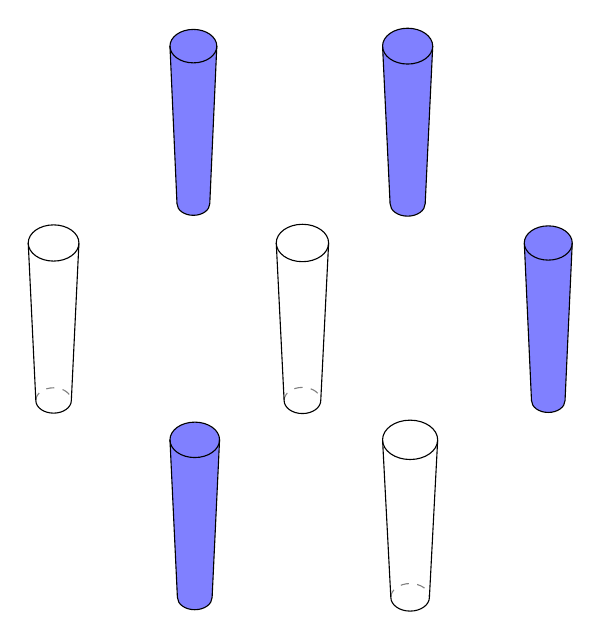
\begin{tikzpicture}
              \pgfdeclarelayer{bg}    % declare background layer
              \pgfdeclarelayer{bbg}    % declare backbackground layer
              \pgfsetlayers{bbg,bg,main}  % set the order of the layers (main is the standard layer)
              \def\height{2}
              \def\primaryRadius{0.35}
              \def\secondaryRadius{.25}
              \def\funneling{0.7}
              \foreach \X/\Y/\F in {1.8/0/0.9, 4.5/0/1, 1.8/5/0.85, 4.5/5/0.91, 3.15/2.5/0.95, 0/2.5/0.92, 6.3/2.5/0.87}
                  {
                  \draw ({\X + (1 - \funneling) * \primaryRadius * \F}, \Y) arc(180:360:{\funneling * \primaryRadius * \F} and {\funneling * \secondaryRadius * \F}) -- (\X + 2 * \primaryRadius * \F, \Y + \height) arc (0:180:{\primaryRadius * \F} and {\secondaryRadius * \F}) -- cycle;
                  \draw (\X + 2 * \primaryRadius * \F, \Y + \height) arc(0:-180: {\primaryRadius * \F} and \secondaryRadius * \F);
                  \begin{pgfonlayer}{bbg}
                      \draw[dashed, gray] ({\X + (1 - \funneling) * \primaryRadius * \F},\Y) arc(180:0:{\funneling * \primaryRadius * \F} and \funneling * \secondaryRadius * \F);
                  \end{pgfonlayer}
                  }
              \begin{pgfonlayer}{bg}
                  \foreach \X/\Y/\F in {1.8/0/0.9,  1.8/5/0.85, 4.5/5/0.91, 6.3/2.5/0.87}
                      {
                      \fill[blue!50] ({\X + (1 - \funneling) * \primaryRadius * \F}, \Y) arc(180:360:{\funneling * \primaryRadius * \F} and {\funneling * \secondaryRadius * \F}) -- (\X + 2 * \primaryRadius * \F, \Y + \height) arc (0:180:{\primaryRadius * \F} and {\secondaryRadius * \F}) -- cycle;
                      }
              \end{pgfonlayer}
          \end{tikzpicture}}
        \pause

        \scalebox{0.38}{
          \tikzsetnextfilename{pore_disorder_2}
          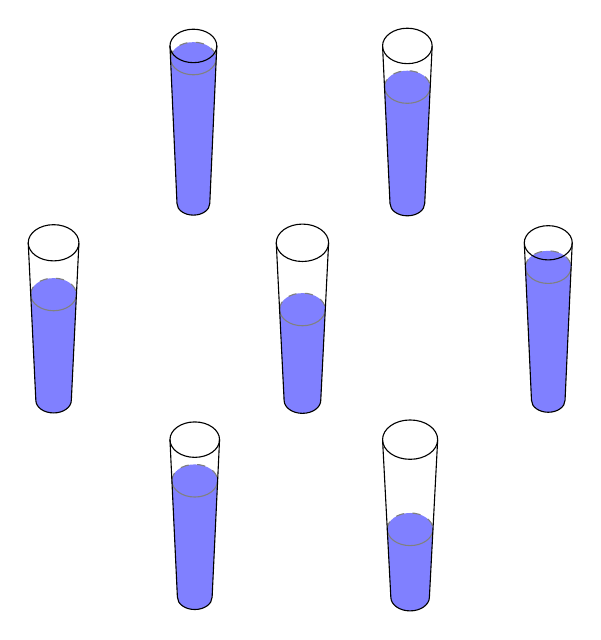
\begin{tikzpicture}
              \pgfdeclarelayer{bg}    % declare background layer
              \pgfdeclarelayer{bbg}    % declare backbackground layer
              \pgfsetlayers{bbg,bg,main}  % set the order of the layers (main is the standard layer)
              \def\height{2}
              \def\primaryRadius{.35}
              \def\secondaryRadius{.25}
              \def\rmax{0.29}
              \def\funneling{0.7}
              \foreach \X/\Y/\F in {1.8/0/0.9, 4.5/0/1, 1.8/5/0.85, 4.5/5/0.9, 3.15/2.5/0.95, 0/2.5/0.92, 6.3/2.5/0.87}
                  {
                  \draw ({\X + (1 - \funneling) * \primaryRadius * \F}, \Y) arc(180:360:{\funneling * \primaryRadius * \F} and {\funneling * \secondaryRadius * \F}) -- (\X + 2 * \primaryRadius * \F, \Y + \height) arc (0:180:{\primaryRadius * \F} and {\secondaryRadius * \F}) -- cycle;
                  \draw (\X + 2 * \primaryRadius * \F, \Y + \height) arc(0:-180: {\primaryRadius * \F} and \secondaryRadius * \F);
                  \begin{pgfonlayer}{bbg}
                      \draw[dashed, gray] ({\X + (1 - \funneling) * \primaryRadius * \F},\Y) arc(180:0:{\funneling * \primaryRadius * \F} and \funneling * \secondaryRadius * \F);
                  \end{pgfonlayer}
                  %
                  \begin{pgfonlayer}{bg}
                      \fill[blue!50] ({\X + \primaryRadius * \F - \rmax}, {\Y + 3.35 * ((\rmax - \F * \funneling * \primaryRadius) * \height / \F / \primaryRadius}) arc(-180:-360:{\rmax} and {\rmax * \secondaryRadius / \primaryRadius}) -- ({\X + (1 - \funneling) * \primaryRadius * \F + 2 * \primaryRadius * \F * \funneling}, \Y) arc (0:-180:{\funneling * \primaryRadius * \F} and {\funneling * \secondaryRadius * \F});
                      \draw[gray, dashed, thin] ({\X + \primaryRadius * \F - \rmax}, {\Y + 3.35 * ((\rmax - \F * \funneling * \primaryRadius) * \height / \F / \primaryRadius}) arc(-180:-360:{\rmax} and {\rmax * \secondaryRadius / \primaryRadius});
                      \draw[gray, thin] ({\X + \primaryRadius * \F - \rmax}, {\Y + 3.35 * ((\rmax - \F * \funneling * \primaryRadius) * \height / \F / \primaryRadius}) arc(180:360:{\rmax} and {\rmax * \secondaryRadius / \primaryRadius});
                  \end{pgfonlayer}
                  }
          \end{tikzpicture}}
    \end{columns}
  \end{frame}
\end{document}
